\section{Project introduction}

\begin{frame}
    \frametitle{Machine Learning Pipeline}
    \begin{figure}[h]
        \centering
        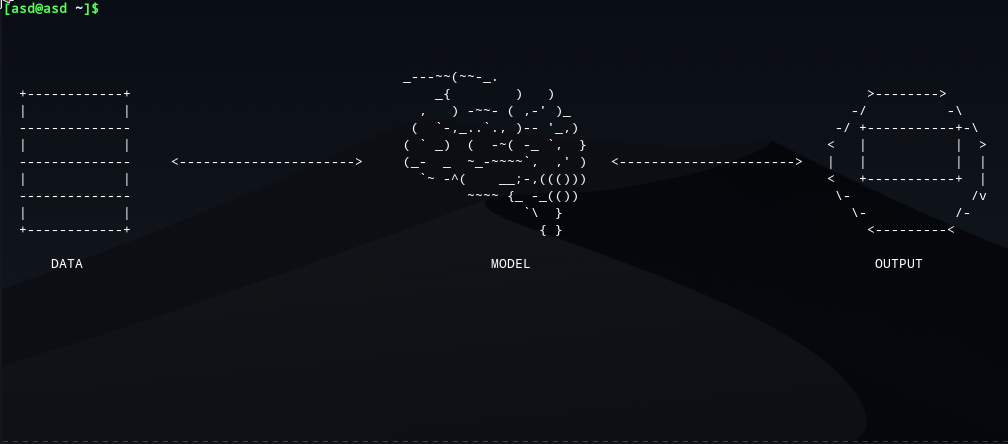
\includegraphics[scale=0.38]{ml_pipeline.png}
         \caption{High-level machine learning pipeline}
    \end{figure}
\end{frame}

\begin{frame}{Anomaly detection using privacy-preserving, synthetic time series data}
    
    \begin{itemize}
        \item Problem
        \begin{itemize}
            \item ML models are very data hungry.
            \item In many cases sharing data comes with privacy risks.
        \end{itemize}
        \item Solution:
        \begin{itemize}
            \item Promising solution: \alert{synthetic data} with privacy guarantees!
            \item Synthetic data with \alert{differential private} (DP) guarantees is a promising solution to ensure privacy independent of downstream task.
        \end{itemize}
        \item BUT:
        \begin{itemize}
            \item \alert{Privacy-Utility-Tradeoff}: Commonly, a gain in privacy results in a loss of utility. 
            \item For \alert{anomaly detection} this might not be the case (?).
        \end{itemize}
    \end{itemize}
    Goal: generate useful and privacy-preserving ECG data for anomaly detection (heartbeat arrhythmia).
\end{frame}


\begin{frame}{Structure}
    \begin{enumerate}
        \item Train baseline model for anomaly detection only on regular heartbeat data using an LSTM-AE.
        \item Generate heartbeat data (without DP) using two approaches:
        \begin{itemize}
            \item[--] AE-MERF
            \item[--] RTSGAN
        \end{itemize}
        \item Train LSTM-AE for anomaly detection on synthetic data and test on real (TSTR).
        \item Add DP noise and repeat:
        \begin{itemize}
            \item[--] AE-DPMERF
            \item[--] DP-RTSGAN
        \end{itemize}
        \item Contaminate training data with anomalous heartbeats and repeat
    \end{enumerate}
\end{frame}


